\section{Modulacja}

\subsection{Dlaczego potrzebujemy modulacji?}

Modulacja cyfrowa to technika zamiany bitów na sygnał oraz sygnału na bity. Jest kluczowym zagadnieniem w przesyle danych pomiędzy systemami komputerowymi. W odróżnieniu od modulacji analogowej, gdzie przesyłane dane wybierane są z przedziału,
modulacja cyfrowa operuje na dyskretnym zbiorze danych (bitach).

Dane reprezentowane są w postaci zmiany parametrów przesyłanego sygnału. Wyróżniane są cztery podstawowe metody:

\begin{enumerate}
    \item PSK (phase-shift keying) --- zmiana fazy fali nośnej sygnału
    \item FSK (frequency-shift keying) --- zmiana częstotliwości fali nośnej sygnału
    \item ASK (amplitude-shift keying) --- zmiana amplitudy fali nośnej sygnału
    \item QAM (quadrature amplitude modulation) --- połączenie PSK oraz FSK, a więc zmieniana jest zarówno amplituda oraz faza
\end{enumerate}

Zmiany sygnału (symbole) kodujące kolejne bity wybierane są ze skończonego zbioru nazywanego alfabetem modulacji.
Dział ten przedstawi popularne techniki modulacji w technologiach Ethernetowych.

\subsection{Wprowadzenie}

Aby ławiej zrozumieć ideę stojącą za bardziej skomplikowanymi technikami modulacji, należałoby na wprowadzeniu wyjaśnić kilka podstawowych pojęć.

Główną charakterystyką łącza jest szerokość pasma (ang. bandwidth) --- określa ona maksymalną (teoretyczną) liczbę bitów jaką łączę jest w stanie przesłać w danym czasie. Podawana jest ona w bitach na sekundę [$bps$] lub w hercach [Hz].

Przepustowość (ang. channel capacity) --- rzeczywista szerokość pasma, zmierzona w określonych warunkach.

Przepływność (ang. bit rate) --- rzeczywista ilość bitów transmitowanych w jednostce czasu poprzez kanał, podawana również w $bps$ lub Hz. Jest stałą charakterystyką danego łącza.

W 1924 roku, Harry Nyquist przedstawił światu równanie, za pomocą którego określić można maksymalną przepływność łącza o szerokości pasma $B$ z wykorzystaniem $V$ poziomów:

\begin{align*}
    \text{Przepływność}_{max} &= 2B * log_{2}{V}
\end{align*}

24 lata później, Claude Shannon rozszerzył równanie Nyquista, uwzględniając szum. Udowodnił on, że maksymalną przepływność łącza, o szerokości pasma $B$ oraz stosunku sygnału do szumu $S/N$, można
obliczyć ze wzoru:

\begin{align*}
    \text{Przepływność}_{max} &= B * log_{2}{(1 + S/N)}
\end{align*}

Granica ta nazywana jest limitem Shannona.

Innym ważnym pojęciem jest multipleksacja (ang. multiplexing) i oznacza przesył wielu symboli jednocześnie w jednym kanale --- realizowany w postaci kilku przewodów, na które dane podawane są jednocześnie w każdym cyklu zegara.

\subsection{Non-Return-to-Zero}

Na początku rozważmy przykład. Najprostszą metodą byłoby używanie dodatniego napięcia dla bitu równego 1 i ujemnego napięcia dla 0.
Technika ta nosi nazwę \textbf{NRZ (Non-Return-to-Zero)}. Nie jest ona wykorzystywana w praktyce --- nadając naprzemiennie 1 i 0 otrzymamy okres równy 2 bity, co oznacza że potrzebujemy pasma B/2 Hz przy prędkości B bit / s.
Nie trudno zauwarzyć, że do szybszego nadawnia, zwiększona musi zostać szerokość pasma, co nie jest optymalnym rozwiązaniem z uwagi na ograniczoność tego zasobu \cite{Computer-networks-Tanenbaum}.

Jednym z rozwiązań tego problemu jest wykorzystanie większej ilości poziomów napięcia. W powyższym przykładzie zastosowane zostały dwa poziomy, a co za tym idzie mamy do dyspozycji dwa symbole przesyłane przez kanał.
Zwiększenie poziomów do 4 dałoby nam 4 różne symbole, a więc 2 bity informacji. W rezultacie przepływność wzrosła dwukrotnie, natomiast szerokość pasma nie zmieniła się. Technika zadziała pod warunkiem, że strona odbiorcza dysponuje sprzętem, który pozwoli jej na
rozróżnienie wielu poziomów napięcia. Jednakże w praktyce jest to koszt, który jesteśmy w stanie ponieść.

\subsection{Pulse-Amplitude Modulation}

Pulse-Amplitude Modulation (PAM) jest najpopularniejszą techniką modulacji wykorzystywaną w technologiach Ethernetowych. Można ją również zobaczyć w innych technologiach (USB4, PCI Express 6.0). Jest to rodzaj modulacji, w którym dane przesyłane jako zmiany amplitudy sygnału. Modulacje PAM można podzielić na dwie kategorię:

\begin{enumerate}
    \item single polarity PAM --- do sygnału dodawana jest stała składowa, aby wartości napięcia były dodatnie
    \item double polarity PAM --- wartości mogą być ujemne lub dodatnie
\end{enumerate}

Modulacja PAM pozwala na przesył więcej niż jednego bitu w jednym takcie zegara, dzięki czemu zgodnie z równaniem Nyquista, zwiększona może zostać przepustowość przy niezmienionej szerokości pasma.
Poszczególne techniki PAM różnią się między sobą liczbą wykorzystywanych poziomów modulacji. Liczba możliwych poziomów jest nieograniczona, jednak wraz ze wzrostem liczby poziomów, różnica pomiędzy symbolami maleje --- a to utrudnia stronie odbiorczej odczyt symboli. Dlatego właśnie rodzaj modulacji PAM wybiera się na podstawie możliwości strony nadawczej i odbiorczej. W systemach wbudowanych czy technologiach automotive wykorzystywanych jest mniej poziomów,
ponieważ w tych przypadkach liczy się kompaktowość, a przepływ danych nie jest duży. Zupełnie odwrotnie jest w technologiach Gigabit Ethernet, gdzie nie ma tak restrykcyjnych ograniczeń sprzętowych, a danych do przesyłu jest dużo.

\subsubsection{PAM3}

PAM3 --- trzypoziomowa modulacja PAM --- do przesyłu wykorzystuje wartości $+1$, $0$, $-1$. Jeden symbol koduje $log_{2}{3} \approx 1,58 \text{ bit/symbol}$.
PAM3 użyty został m.in. w standardach 100BASE-T4 (wczesna implementacja Fast Ethernet) i BroadR-Reach Ethernet standard --- wykorzystywany w branży automotive, opracowany przez firmę Broadcom Corporation.
Nie jest to schemat modulacji PAM, który często pojawia się w praktycznych rozwiązaniach, z uwagi na to, że technologie wykorzystujące tą technikę nie zostały szeroko przyjęte.

Ciekawym aspektem jest podział bitów na symbole. Na pierwszy rzut oka widać, że istnieje problem z grupowaniem bitów --- nie można przecież przesłać $1,58$ bita. W modulacjach z liczbą poziomów będącą potęgą $2$ podział jest bardzo prosty --- bity grupujemy w dwójki, czwórki \dots i bezpośrednio mapujemy na symbole.

Tutaj rozwiązaniem jest tymczasowa zamiana bitów na trity (system trójkowy). Przykładowo, w wersji drugiej USB4, dane dzieli się 11-bitowe grupy po czym każda z nich zamienana jest na 7 tritów, osiągając przy tym
efektywność rzędu $\frac{11/7}{log_{2}{3}} * 100\% \approx 99\% $


\subsubsection{PAM4}

PAM4 --- czteropoziomowa modulacja PAM --- do przesyłu wykorzystuje wartości $3$, $1$, $-1$, $-3$, które kolejno odpowiadają logicznym wartościom 11, 10, 01, 00. W porównaniu do NRZ (Non-Return-to-Zero) ma przewagę posiadania dwukrotnie większej przepływność przy tej samej prędkości transmisji, co ilustruje poniższy rysunek \cite{Intel-pam4}:

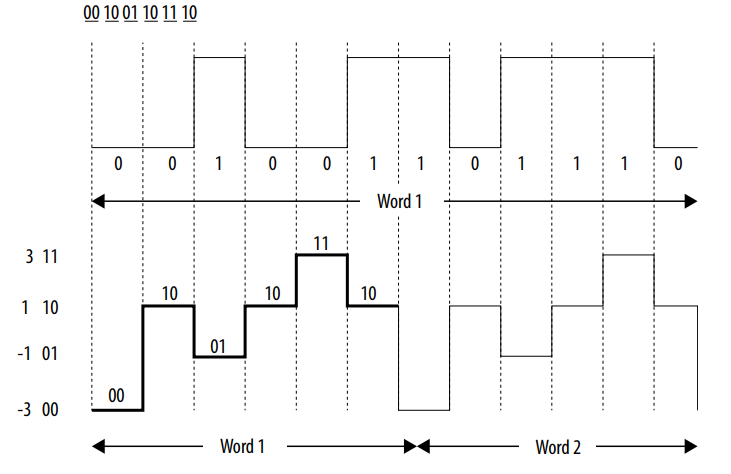
\includegraphics[scale=0.5]{pam4_vs_nrz.png}

Warto zwrócić uwagę, że w NRZ mamy jedno narastające zbocze ($0 \rightarrow 1$) i jedno opadające zbocze ($1 \rightarrow 0$), co daje dwie zmiany napięcia. W przypadku PAM4 jest to 6 narastających zbocz
($00 \rightarrow 01, 00 \rightarrow 10, 00 \rightarrow 11, 01 \rightarrow 10, 01 \rightarrow 11, 10 \rightarrow 11$) oraz 6 opadających zbocz
($11 \rightarrow 10, 11 \rightarrow 01, 11 \rightarrow 00, 10 \rightarrow 01, 10 \rightarrow 00, 01 \rightarrow 00$), które łącznie dają 12 różnych zmian napięcia.
Ma to znaczący wpływ na stosunek sygnału do szumu (SNR).

PAM4 wykorzystywany jest m.in. w technologiach 100, 200 i 400 Gigabit Ethernet.

\subsubsection{PAM16}

PAM16 --- szesnastopoziomowa modulacja PAM --- analogicznie do poprzednich przypadków wykorzystuje wartości $15$, $13$, $11$, \dots , $1$, $-1$, $-3$, \dots , $-13$, $-15$. Szesnaście poziomów daje 4 bity na symbol. Wykorzystywana jest w technologiach 10GBASE-T, 25GBASE-T czy 40GBASE-T.